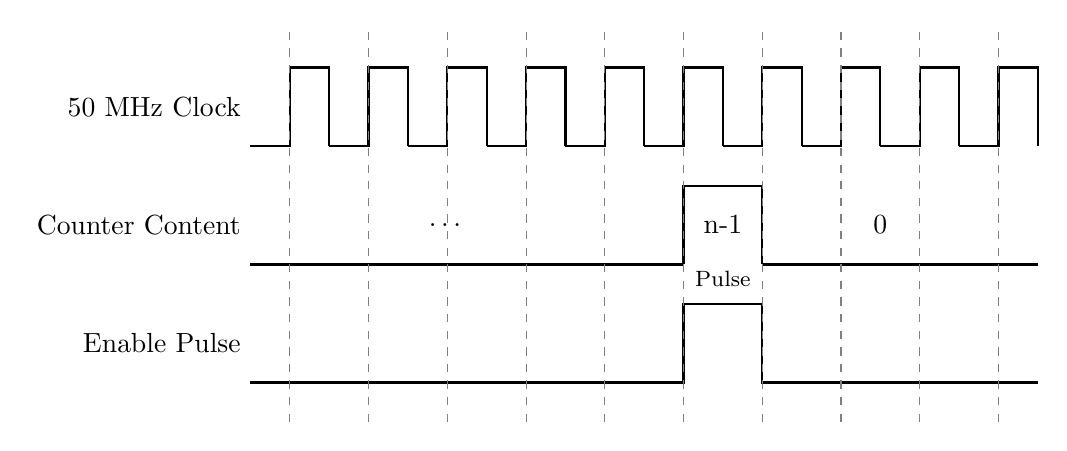
\begin{tikzpicture}[
    signal/.style={draw, thick},
    axis/.style={draw, ->},
    dashed_line/.style={draw, dashed, gray}
]
    % Define coordinates
    \def\clkY{3}
    \def\cntY{1.5}
    \def\enY{0}
    
    % Labels
    \node[left] at (0, \clkY + 0.5) {50 MHz Clock};
    \node[left] at (0, \cntY + 0.5) {Counter Content};
    \node[left] at (0, \enY + 0.5) {Enable Pulse};

    % Clock Signal (Rising edges at 0.5, 1.5, ...)
    \foreach \x in {0, 1, 2, 3, 4, 5, 6, 7, 8, 9} {
        \draw[signal] (\x, \clkY) -- (\x+0.5, \clkY) -- (\x+0.5, \clkY+1) -- (\x+1, \clkY+1) -- (\x+1, \clkY);
    }

    % Counter Content (Updates on rising edge at 5.5 and 6.5)
    \draw[signal] (0, \cntY) -- (5.5, \cntY);
    \node at (2.5, \cntY+0.5) {\dots};
    \draw[signal] (5.5, \cntY) -- (5.5, \cntY+1) -- (6.5, \cntY+1) -- (6.5, \cntY);
    \node at (6, \cntY+0.5) {n-1};
    \draw[signal] (6.5, \cntY) -- (10, \cntY);
    \node at (8, \cntY+0.5) {0};

    % Enable Pulse (High when counter is n-1, aligned with rising edges)
    \draw[signal] (0, \enY) -- (5.5, \enY) -- (5.5, \enY+1) -- (6.5, \enY+1) -- (6.5, \enY) -- (10, \enY);

    % Dashed vertical lines at rising edges
    \foreach \x in {0.5, 1.5, 2.5, 3.5, 4.5, 5.5, 6.5, 7.5, 8.5, 9.5} {
        \draw[dashed_line] (\x, -0.5) -- (\x, \clkY+1.5);
    }
    
    \node[above, font=\footnotesize] at (6, \enY+1.1) {Pulse};

\end{tikzpicture}
